%encoding UTF-8
\author{Евгений Синельников, Игорь Чудов}
\city{Саратов}
\affiliation{Базальт СПО}
\projecttitle{Стажёрская программа компании "Базальт СПО"}
\projecturl{\url{http://altlinux.org/}}
\title{Приобщение к участию в разработке свбодных программ на примере
стажировки в компании Базальт СПО}
\maketitle

\begin{abstract}
  В рамках доклада рассмотрена проблема обучения новых
  сотрудников в компаниях, работающих с СПО. Предложены методики для
  ускорения процедуры включения людей в рабочие процессы. Представлены
  примеры вводных документов.
\end{abstract}


\section{Проблематика}

В сравнении с компаниями, ориентированными на outsource-разработку для
множества различных заказчиков, небольшие продуктовые компании, особенно
если они связаны с разработкой СПО, испытывают дефицит кадров.

В качестве примера предлагается рассмотреть выборку заявок на Join
с сайта \url{http://bugzilla.altlinux.org/} за весь доступный период
(2008-2020 годы):

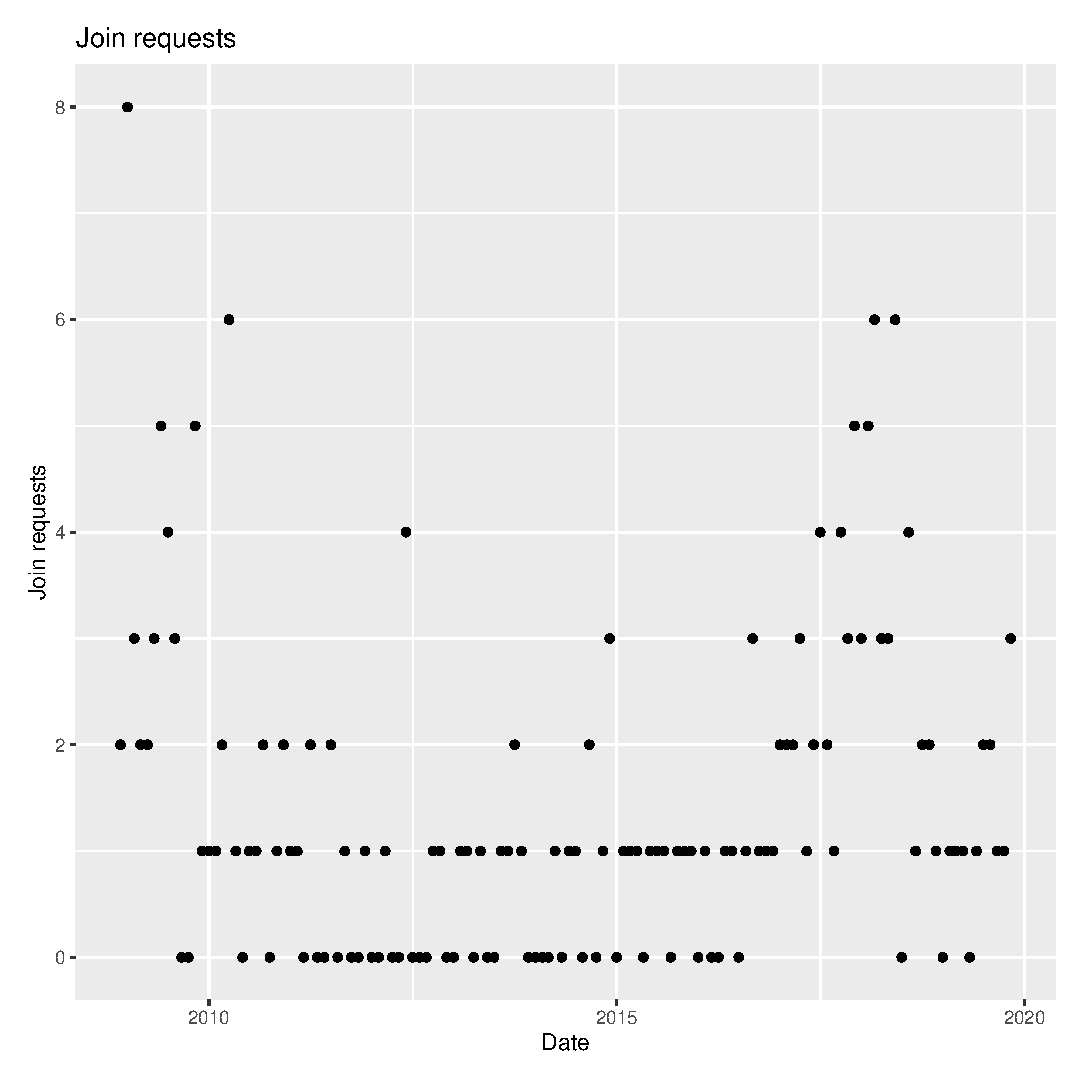
\includegraphics[width=\textwidth,height=\textheight,keepaspectratio]{ggplot}

Данные представляют из себя формальную характеристику потока
потенциальных сотрудников. Не смотря на длительный период выборки можно
отметить, что количество поступающих заявок невелико, что может служить
сигналом о нескольких проблемах (при рассмотрении вопроса извне):

\begin{itemize}
\item проблема с процедурой подачи заявок (неочевидность, сложность,
бюрократия, длительность);
\item проблема с методом коммуникации (устаревание инструмента и
методики, недостаточность усилий по преодолению барьеров коммуникации);
\item также сказывается специфика предметной области с которой связана
работа.
\end{itemize}

Со стороны же тех, кто вовлечён в работу с СПО, инструменты коммуникации
типа IRC, e-mail и других подобных представляют ценность за счёт:

\begin{itemize}
\item доступность на разных платформах;
\item широкая аудитория со всего мира;
\item надёжность, стабильность во времени;
\item простота.
\end{itemize}

В связи с неоднозначным восприятием ситуации разными группами людей
возникает конфликт интересов. Для решения этой проблемы компаниям,
работающим с СПО, приходится находить способы транслировать свою
культуру в массы с целью формирования сообщества, разделяющего эти
ценности. В противном случае работодатель сталкивается с дефицитом
кадров, который не может восполнить за счёт основной массы рынка
рабочей силы так как требуемый для работы с СПО уровень квалификации на
данный момент таков, что сотрудник способен достичь его только в том
случае, если он взаимодействует с СПО не только в рамках должностных
обязанностей.

Для снятия части нагрузки с основых сотрудников, а также для
наработки опыта передачи знаний и культурных ценностей, в Саратовском
офисе компании "Базальт СПО" была организована стажёрская программа.

Для участия в стажёрской программе была размещена заявка на HeadHunter
со следующими результатами:

\begin{itemize}
\item 28 входящих заявок получено;
\item из них 6 человек отправили свои резюме и пришли на собеседование;
\item из 6 человек было отобрано 4 стажёра;
\item один стажёр отказался от работы через 4 дня.
\end{itemize}

Наблюдаемая по заявке ситуация оказалась такова: Поступающие кадры
незнакомы с требуемыми инструментами, а также не воспринимают принятые
в сообществе разработчиков СПО средства коммуникации.

\section{Методика преодоления проблемы}

В процессе жизнедеятельности человек связанный с СПО проходит несколько
стадий:

\begin{itemize}
\item пользователь - использует СПО в повседневной деятельности;
\item разработчик - пишет СПО (возможно, на коммерческой основе);
\item мейнтейнер - не только пишет СПО, но и внедряет его в открытые
продукты/дистрибытивы ОС.
\end{itemize}

В данном случае мейнтейнер рассматривается как высшая ступень эволюции
инженера. Организованная в компании "Базальт СПО" стажёрская программа
преследовала цель прохождения данных этапов за счёт оплачиваемого
вовлечения инженеров в процесс решения задач с использованием СПО за
счёт привлечения людей с рынка труда.

Для стажёров были проведены вводные лекции, определён список задач с
нарастанием их сложности, а также выделено время для помощи с
возникающими вопросами.


\section{Анализ результатов}

В рамках месячной стажировки получены следующие результаты:

\begin{itemize}
\item один из стажёров разработал утилиту ALT Media Writer дополнив и
улучшив один из открытых проектов;
\item второй стажёр занимался тестированием Samba и в результате сильно
продвинул проект разбирая большое количество use-cases;
\item третий стажёр занимался написанием документации к Samba на публичной
Wiki \url{http://www.altlinux.org/}. В результате он получил как
общее понимание проекта, так и сделал его доступнее для русскоязычных 
пользователей;
\item Сотрудники компании получили необычный опыт наставничества и
провели разбор допущенных в процессе ошибок.
\end{itemize}

На основании полученных результатов сделаны выводы:

\begin{itemize}
\item специфика отрасли требует найма сотрудников и стажёров высокой
квалификации;
\item приходящие с рынка кадры в большинстве своём недообучены и
обладают недостаточной квалификацией;
\item работа со стажёрами недостаточной квалификации забирает
непозволительно много времени у основного состава сотрудников, что
понижает рентабельность найма стажёров;
\item найм сотрудников из сообщества может быть несравнимо более
результативен по сравнению с общепринятыми методами, но только при наличии
самого сообщества.
\end{itemize}


\section{Библиография}

\begin{thebibliography}{9}
\bibitem{altbug} ALT Linux Bugzilla \url{http://bugzilla.altlinux.org/}
\bibitem{altwiki} ALT Linux Wiki \url{http://www.altlinux.org/}
\end{thebibliography}


%%% Local Variables: 
%%% mode: latex
%%% TeX-master: "../main"
%%% End: 
